\documentclass[border=4pt]{standalone}
\usepackage{tikz,amsmath}
\usetikzlibrary{arrows.meta}
\definecolor{nuit}{HTML}{190F3C}\definecolor{bleu}{HTML}{3746FF}
\definecolor{corailf}{HTML}{D6455A}
% Tube épais : R_e/R_i = 1,5 ; a = p_i R_i^2/(R_e^2-R_i^2) = 0,8 p_i
\begin{document}
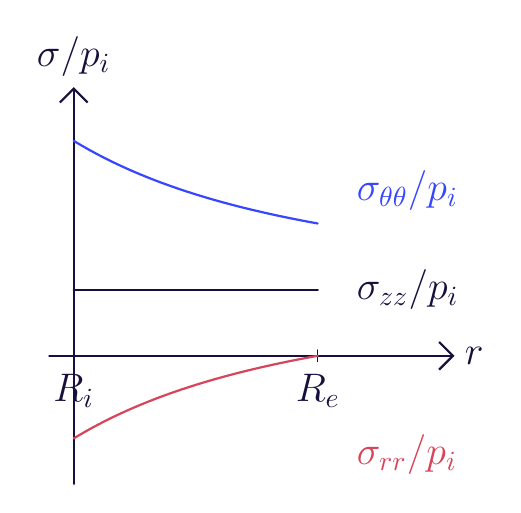
\begin{tikzpicture}[x=6.2cm,y=1.05cm,line cap=round,>={Straight Barb[length=5pt]}]
  \def\a{0.8}\def\Re{1.5}
  % axes
  \draw[->,thick,nuit] (0.95,0) -- (1.78,0) node[right] {\Large $r$};
  \draw[->,thick,nuit] (1,-1.55) -- (1,3.25) node[above] {\Large $\sigma/p_i$};
  \draw[nuit] (\Re,0.07) -- (\Re,-0.07);
  \node[below=3pt,nuit] at (1,0) {\Large $R_i$};
  \node[below=3pt,nuit] at (\Re,0) {\Large $R_e$};
  % courbes
  \draw[thick,bleu,domain=1:\Re,samples=60] plot (\x,{\a*(1+\Re*\Re/(\x*\x))});
  \draw[thick,nuit,domain=1:\Re] plot (\x,{\a});
  \draw[thick,corailf,domain=1:\Re,samples=60] plot (\x,{\a*(1-\Re*\Re/(\x*\x))});
  % étiquettes
  \node[anchor=west,bleu] at (\Re+0.06,2.0) {\Large $\sigma_{\theta\theta}/p_i$};
  \node[anchor=west,nuit] at (\Re+0.06,\a) {\Large $\sigma_{zz}/p_i$};
  \node[anchor=west,corailf] at (\Re+0.06,-1.2) {\Large $\sigma_{rr}/p_i$};
\end{tikzpicture}
\end{document}
